\documentclass[11pt]{article}
\usepackage[letterpaper,margin=1in]{geometry}
\usepackage[T1]{fontenc}
\usepackage{lmodern}
\usepackage{amsmath,amssymb}
\usepackage{graphicx}
\usepackage{booktabs}
\usepackage{caption}
\usepackage[hidelinks]{hyperref}
\usepackage{titlesec}
\titlespacing*{\section}{0pt}{8pt plus 2pt}{3pt}
\captionsetup{font=small,labelfont=bf}
\setlength{\abovecaptionskip}{4pt}
\setlength{\textfloatsep}{10pt}

\begin{document}

\vspace*{-18pt}
\begin{center}
{\large\bfseries Where Evolution Converges and Stalls:\\ A Network Analysis of Snake-like Body Forms in Squamates}\\[4pt]
Henry Ji and Calvin Zhang \quad CS/INFO 6850 \quad Progress report, November 23, 2026
\end{center}

\section{Introduction}

Snake-like bodies, with long trunks and reduced or absent limbs, evolved dozens of times in lizards. The form is rare, yet it keeps reappearing in unrelated lineages. We ask two network questions about this: where do unrelated lineages converge, and which steps of the transformation are slow?

Prior work models how traits change along a phylogeny: dependent evolution of discrete traits (Pagel 1994), pathways on the hypercube of trait combinations (HyperTraPS; Greenbury et al.\ 2020), and the several developmental routes to a snake-like form (Bergmann and Morinaga 2019). Our contribution is not a new evolutionary model. We turn species data into a network and apply the course's tools to it: small-world structure, Cheeger cuts and random walks. A standard trait model only dates and orients changes on the tree, so that walks on the network carry evolution's real direction and timing.

\section{Data}

We merged five sources onto the dated tree of 6,885 squamates of Title et al.\ (2024): a literature compilation of digits, presacral vertebrae and habitat for 1,386 species (Dryad, 2025), vertebral counts for 2,364 species, mostly from radiographs (Dryad, 2026), the limb-reduced skink database of Camaiti et al.\ (2022), Bergmann and Morinaga's (2019) measurements, and SquamBase (Meiri 2024), which records limb status, substrate and biome for every squamate. Where sources overlap they agree closely (vertebral counts, Spearman 0.99 over 1,052 species; digits, 0.98). Uncounted digits are inferred as 10 for ``four well developed limbs'' (right for 96\% of counted species) and 0 for limbless snakes only, since 13\% of lizards called limbless keep vestigial digits. This gives 2,403 species with both counts, 1,451 of them lizards, against 911 in the largest single source.

\section{Methods}

\textit{Species network.} Each of the 1,451 lizards links to its six closest relatives, by the age of their common ancestor, and its six closest look-alikes, by distance in standardized digit count and log vertebral count. Snakes, which share one snake-like ancestor, are left out. A look-alike link between derived species (elongate or with fewer than 10 digits) whose ancestors split over 100 million years ago is a convergence link. We compare clustering and mean path length with a random graph of the same density (Watts and Strogatz 1998).

\textit{Convergence bottleneck.} On the body-form graph with weights $w_{ij} = \exp(-\|z_i - z_j\|^2 / 2h^2)$, cut off at $3h$ with $h = 0.3$, the conductance of a set $S$ is $\phi(S) = w(S, \bar S) / \min(\mathrm{vol}\, S, \mathrm{vol}\, \bar S)$, where $w(S, \bar S)$ is the weight crossing the cut and $\mathrm{vol}\, S$ the total weighted degree in $S$. We take the sweep cut of the Fiedler vector of the normalized Laplacian, which by Cheeger's inequality comes within $\sqrt{2\lambda_2}$ of the best possible (Chung 1997). Bridge species are those carrying 80\% of the weight across the cut, and lineages are groups of species whose ancestry splits more than 50 million years ago.

\textit{Trait walk and time.} Four binary traits describe a body: elongate ($E$, at least 35 presacral vertebrae; fully limbed species average 26), digits reduced ($R$), digitless ($Z$) and burrowing ($F$). Since $Z$ implies $R$, the state graph is the 4-cube minus four nodes. Along each branch a lineage moves on it as a continuous-time Markov chain: trait $i$ is gained at rate $r_i \exp(\sum_j x_j \Gamma_{ji})$ and lost at a shared rate $\mu$, so $e^{\Gamma_{ji}}$ is how much holding $j$ speeds the gain of $i$. Rates are fitted by maximum likelihood over all 6,885 species (Felsenstein pruning). We then sample 100 histories consistent with the data by stochastic mapping (Nielsen 2002; Huelsenbeck et al.\ 2003), count independent origins of a snake-like body ($E$ and $Z$), time each journey from the last ordinary-lizard state, and compute each state's mean stay, the time spent in it divided by the number of departures.

\textit{Biased walks and drivers.} With $\rho_t$ the ratio of gains to losses of trait $t$ in the sampled histories, the biased walk steps from species $i$ to neighbor $j$ with probability proportional to $\prod_t \rho_t^{(x_{jt} - x_{it})/2}$; the unbiased walk picks neighbors uniformly. To back out environmental drivers we add a SquamBase biome (desert and xeric shrubland, or tropical moist forest) as a fifth trait, fitting couplings in both directions so that ``the environment speeds a change'' is separated from ``species with that body move there.'' What-ifs change only how often lineages enter an environment or take up burrowing, and the fitted couplings carry the consequences to the expected time from an ordinary lizard to a snake-like body.

\textit{Uncertainty.} Network intervals (95\%) come from 200 resamples keeping 80\% of species; rate intervals from a normal approximation at the maximum (numerical Hessian), with parameter draws propagated through the maps and walks. Two couplings sit at the bound $e^6 \approx 400$ and are lower bounds.

\begin{figure}[t]
\centering
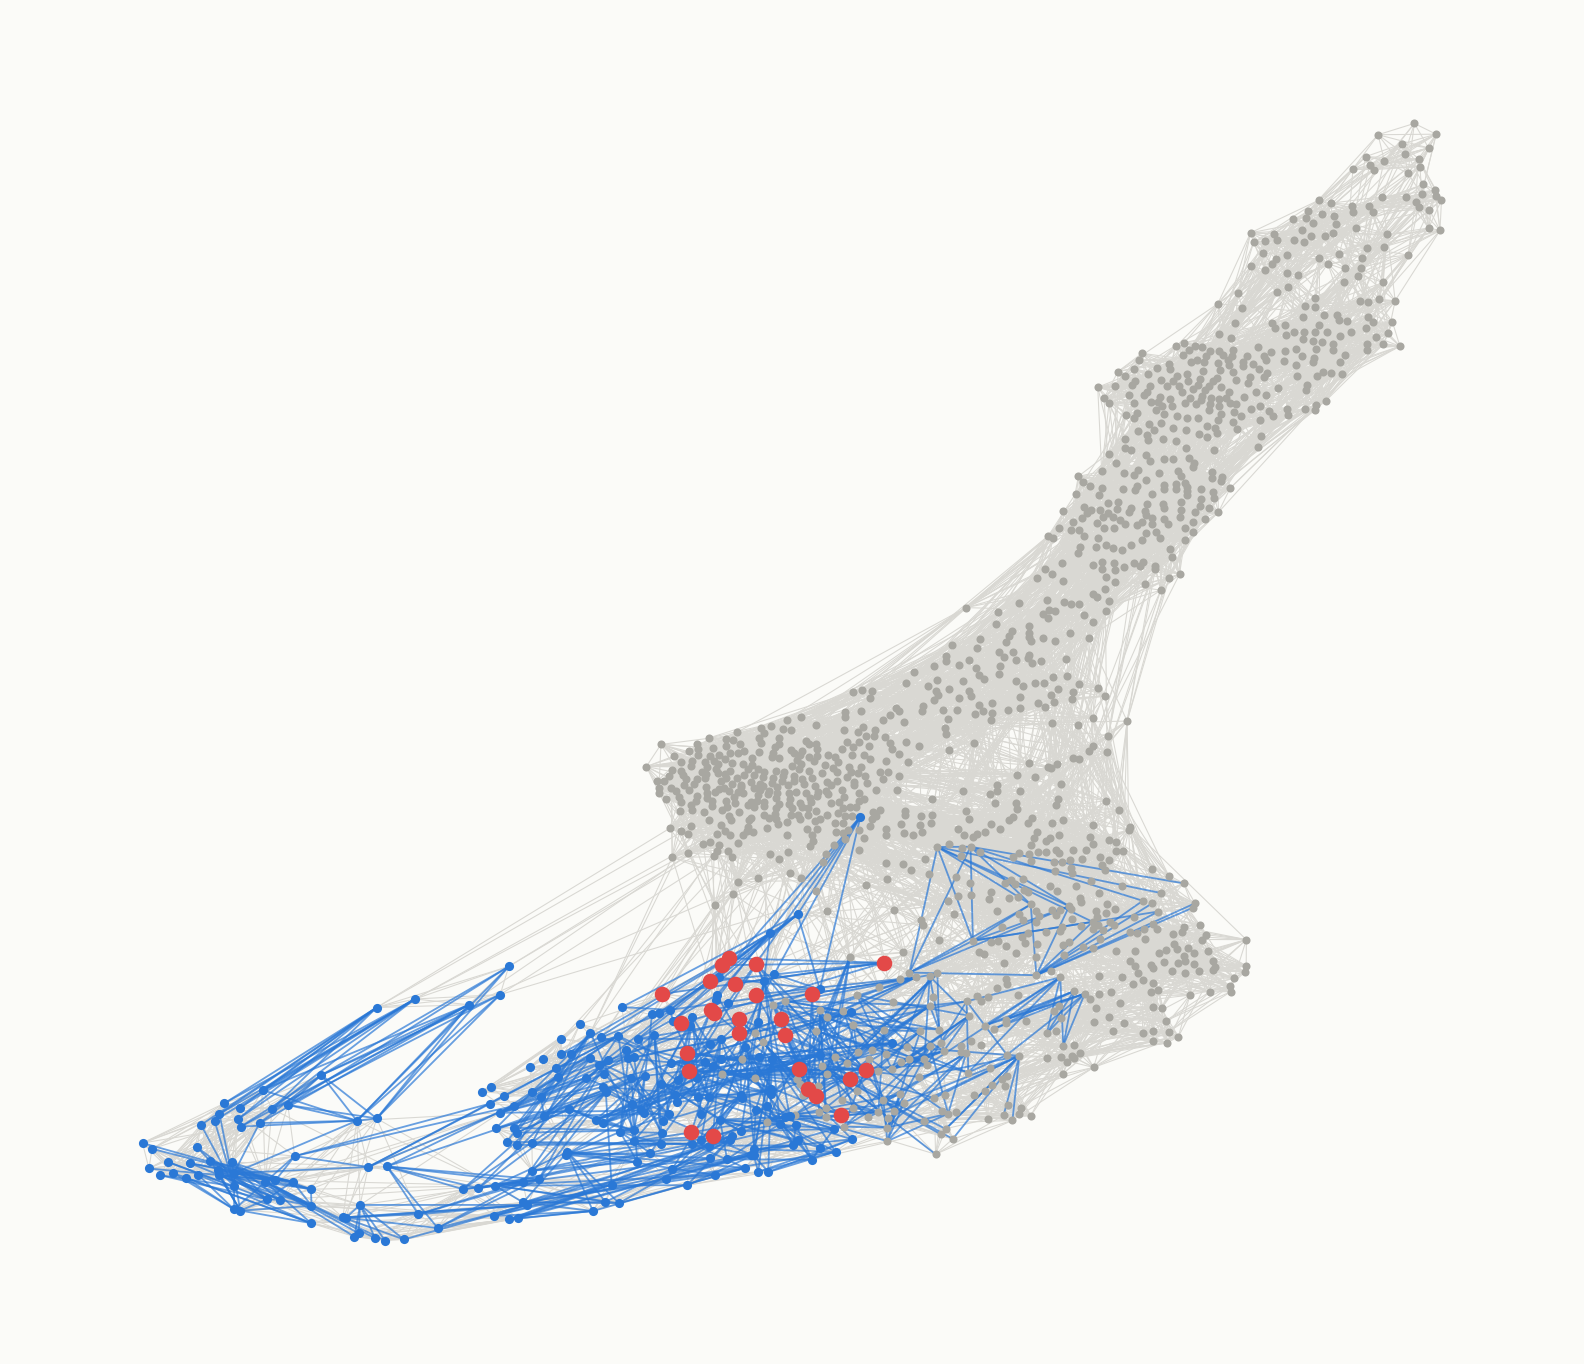
\includegraphics[width=0.3\textwidth]{figures/network.png}\hfill
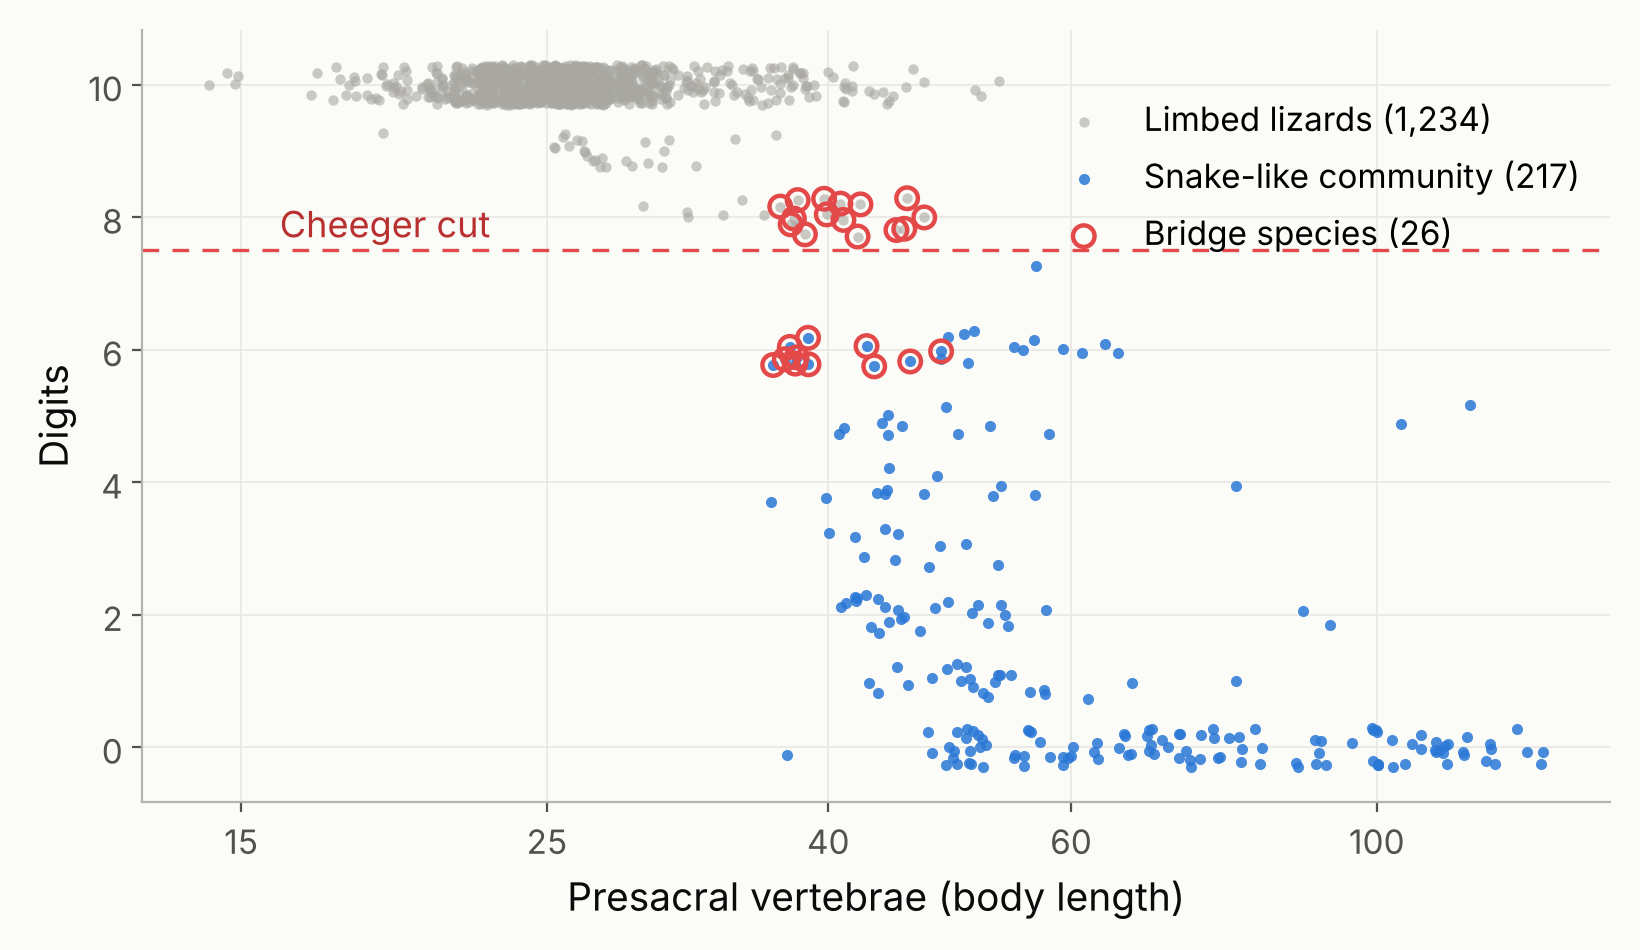
\includegraphics[width=0.47\textwidth]{figures/cut.png}
\caption{Left: the species network of 1,451 lizards, laid out by force direction. Grey nodes are limbed lizards, blue nodes the snake-like side of the Cheeger cut, blue edges convergence links, and red nodes the bridge species. Right: the same species in the plane of vertebral count and digits; the dashed line is the cut, and the bridge species sit at 6 to 8 digits, where few species live.}
\label{fig:network}
\end{figure}

\section{Results}

The network is a small world: clustering is 18 times that of a random graph of the same density (15 to 17 times in every 80\% subsample), while mean paths are only 1.39 times longer. The relatives alone fall into 45 pieces, and 720 convergence links between species over 100 million years apart act as the long-range shortcuts that knit them together.

The body-form network has one sharp bottleneck (Figure~\ref{fig:network}): a Cheeger cut of conductance 0.003 (0.002 to 0.004), against 0.38 for the best cut among limbed lizards. On one side sit 217 snake-like lizards from 15 families and about 30 independent lineages, so unrelated lineages converge on one region of the network. Only 26 bridge species from 6 lineages span the cut: \textit{Lerista}, \textit{Brachymeles}, \textit{Bachia}, \textit{Hemiergis}, \textit{Chalcides} and \textit{Saiphos}, the genera biologists already study as natural experiments in limb loss, found here without labels. The same cut appears in all 200 resamples, with snakes added, and on the Zheng and Wiens (2016) tree.

The trait model shows why the bottleneck is thin. Directed couplings are strongly supported over independent traits (likelihood ratio, $p \approx 10^{-130}$): burrowing speeds elongation and digit reduction about 16-fold, elongation and digit reduction speed each other 14 to 18-fold, and elongation and complete digit loss each speed the other at least 400-fold. An ordinary lizard lineage waits 510 million years (447 to 566) on average before any change begins, longer than the 206 million years squamates have existed, but once started it becomes snake-like in 36 million years (33 to 41). This happened about 47 separate times (43 to 54), with elongation before any digit loss in 71\% of journeys (57 to 86\%).

Evolution's walk is biased toward the snake-like form. Each trait was gained 1.9 to 7.1 times more often than lost, and the walk tilted by these ratios reaches the snake-like community in 60 steps instead of 156, a speedup of 2.6 (2.4 to 2.8). Of the environments tested, only burrowing drives the change (Figure~\ref{fig:drivers}). Desert and moist forest speed no body change; their links run the other way, with elongate lineages moving into deserts (2.8-fold, 1.4 to 5.6) and digitless ones into forests (6.2-fold, 1.1 to 35). So if lineages took up burrowing twice as often, as surface habitat loss might cause, snake-like bodies would arrive 25\% sooner (18 to 31\%); if soil degradation halved it, 24\% later (16 to 36\%). Doubling entry into deserts or exit from forests changes this by at most 7\%.

\begin{figure}[t]
\centering
\begin{minipage}[c]{0.46\textwidth}
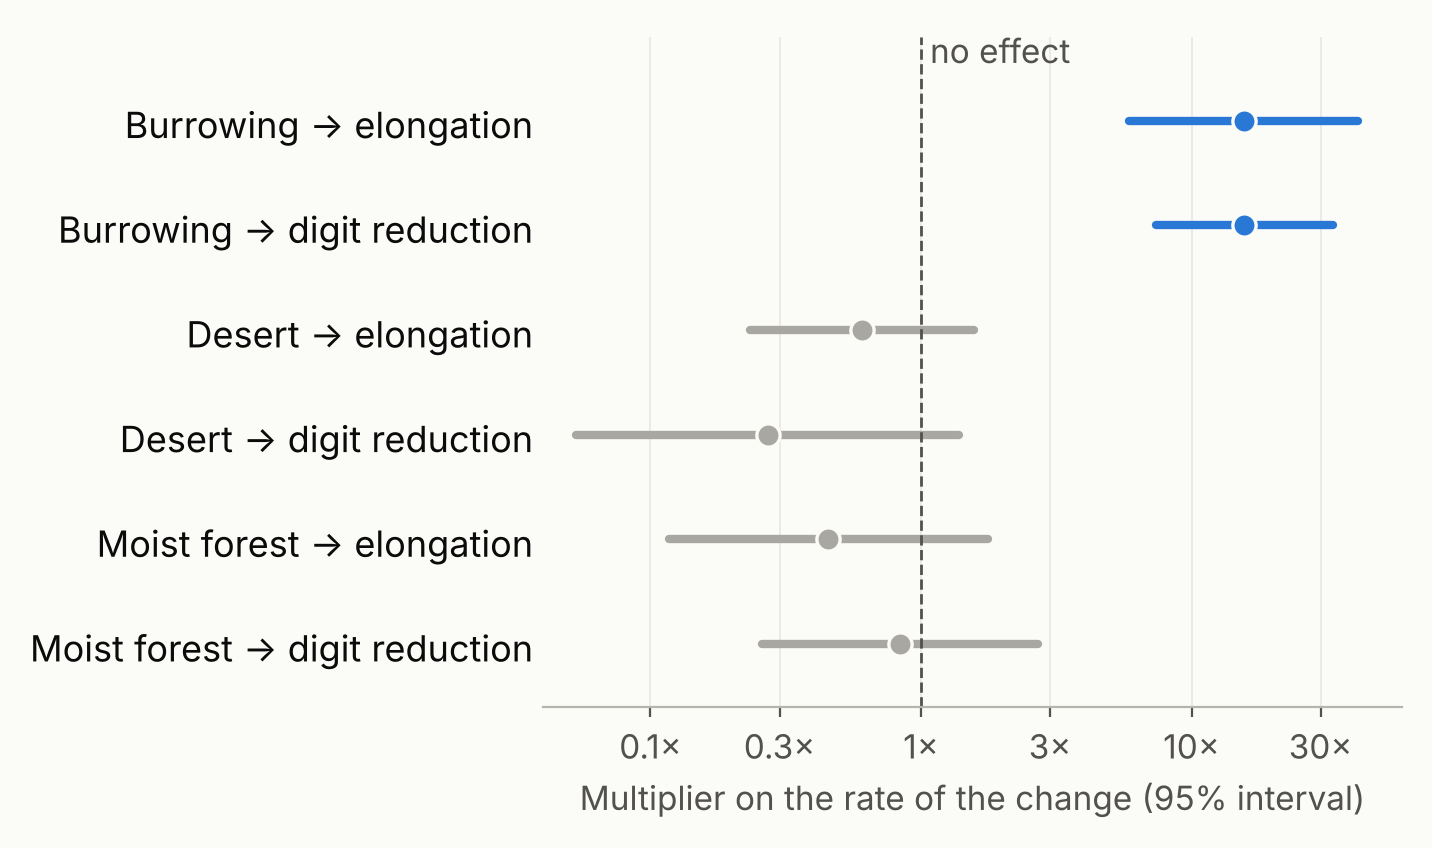
\includegraphics[width=\textwidth]{figures/drivers.png}
\end{minipage}\hfill
\begin{minipage}[c]{0.47\textwidth}
\small
\begin{tabular}{@{}lr@{}}
\toprule
Quantity & Estimate (95\% interval) \\
\midrule
Cut conductance & 0.003 (0.002--0.004) \\
Clustering vs random & 18$\times$ (subsamples 15--17) \\
Ordinary-lizard stay & 510 Myr (447--566) \\
Start to snake-like & 36 Myr (33--41) \\
Independent origins & 47 (43--54) \\
Biased walk speedup & 2.6$\times$ (2.4--2.8) \\
Burrowing $\to$ elongation & 16$\times$ (6--41) \\
Burrowing twice as often & $-25\%$ ($-31$ to $-18$) \\
Burrowing half as often & $+24\%$ ($+16$ to $+36$) \\
\bottomrule
\end{tabular}
\end{minipage}
\caption{Left: environmental drivers backed out from the tree, as multipliers on the rate of each change with 95\% intervals; only burrowing excludes no effect. Right: key results with 95\% intervals.}
\label{fig:drivers}
\end{figure}

\section{Discussion and next steps}

Snake-like bodies are hard to start and quick to finish. A high barrier at the ordinary-lizard state makes the form rare, strong coupling after the first step makes lineages that start finish the same way, and the network shows the result as one thin cut with many unrelated lineages beyond it and almost nobody in between. Limitations remain: binary thresholds compress continuous traits, digit counts are missing for about 500 lizards, intervals rest on a normal approximation, biome is a coarse proxy for environment, and the what-ifs are counterfactuals, not forecasts. Next we will repeat the analysis on 100 alternative trees, use counted digits and vertebrae to give the walk hundreds of body forms, test species-level climate as a driver, and add a second group.

\vspace{4pt}
\noindent{\footnotesize\textbf{References.}
Bergmann, P.\,J.\ and Morinaga, G.\ (2019). The convergent evolution of snake-like forms by divergent evolutionary pathways in squamate reptiles. \textit{Evolution}.
Camaiti, M.\ et al.\ (2022). A database of the world's limb-reduced skinks. \textit{Journal of Biogeography} 49, 1397--1406.
Chung, F.\ (1997). \textit{Spectral Graph Theory}. AMS.
Greenbury, S.\,F., Barahona, M.\ and Johnston, I.\,G.\ (2020). HyperTraPS: inferring probabilistic patterns of trait acquisition. \textit{Cell Systems} 10, 39--51.
Huelsenbeck, J.\,P., Nielsen, R.\ and Bollback, J.\,P.\ (2003). Stochastic mapping of morphological characters. \textit{Systematic Biology} 52, 131--158.
Meiri, S.\ (2024). SquamBase: a database of squamate (Reptilia: Squamata) traits. \textit{Global Ecology and Biogeography} 33.
Nielsen, R.\ (2002). Mapping mutations on phylogenies. \textit{Systematic Biology} 51, 729--739.
Pagel, M.\ (1994). Detecting correlated evolution on phylogenies. \textit{Proceedings of the Royal Society B} 255, 37--45.
Title, P.\,O.\ et al.\ (2024). The macroevolutionary singularity of snakes. \textit{Science}.
Watts, D.\,J.\ and Strogatz, S.\,H.\ (1998). Collective dynamics of small-world networks. \textit{Nature} 393, 440--442.
Zheng, Y.\ and Wiens, J.\,J.\ (2016). A time-calibrated phylogeny for squamate reptiles based on 52 genes and 4162 species. \textit{Molecular Phylogenetics and Evolution} 94, 537--547.
Datasets: Dryad doi:10.5061/dryad.crjdfn3g7 (2025); doi:10.5061/dryad.4qrfj6qr1 (2026); doi:10.5061/dryad.76hdr7t3b (2024); doi:10.5061/dryad.5rh14nc (2019).}

\end{document}
